\begin{pastexam}[label={px:df3-110-ds-01}]{地方三等資訊處理 110 年 第一題}
（申論；25 分）

\begin{itemize}[leftmargin=2.2em]
\item[㈠] 請分別寫出下圖二元樹的前序走訪法（preorder traversal）、中序走訪法（inorder traversal）、後序走訪法
（postorder traversal）的結果（6 分）
\item[㈡] 請在無法預知二元樹的節點數條件下，設計在程式中表示二元樹的資料結構。再假設二元樹已依前述結構儲存在
程式，設計一副程式（或函式）的演算法，在提供樹根給此副程式（或函式）後，其執行二元樹中序走訪法的程序並輸出
走訪結果。此副程式（或函式）不可使用遞迴呼叫技術但可添加其他資料結構，演算法的時間複雜度和空間複雜度須均為
O(n)，n 為二元樹的節點個數。演算法可以虛擬碼（pseudo-code）或以高階語言如 C 呈現。需分析說明副程式（或函式）
演算法的時間複雜度和空間複雜度均為 O(n)。（提醒：若用遞迴呼叫技術設計，演算法部分不給分）（13 分）
\item[㈢] 請分別說明在程式執行過程，以第㈡子題非遞迴呼叫技術設計相較於以遞迴呼叫技術設計在時間與空間的效能優勢
各為何？（6 分）
\end{itemize}
\begin{center}
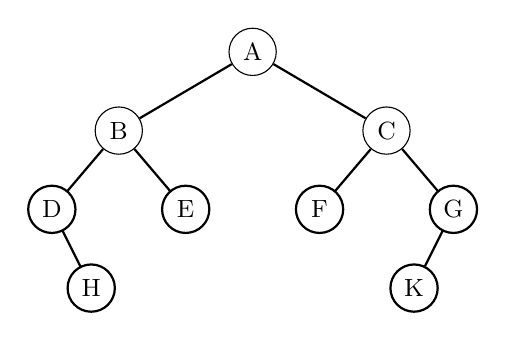
\begin{tikzpicture}[v/.style={circle,draw,minimum size=6mm,inner sep=0pt,font=\small},
  edge from parent/.style={draw,thick},
  level distance=10mm, level 1/.style={sibling distance=34mm}, level 2/.style={sibling distance=17mm},
  level 3/.style={sibling distance=10mm}]
\node[v] {A}
  child {node[v] {B}
    child {node[v] {D} child[missing] {} child {node[v] {H}}}
    child {node[v] {E}}}
  child {node[v] {C}
    child {node[v] {F}}
    child {node[v] {G} child {node[v] {K}} child[missing] {}}};
\end{tikzpicture}
\end{center}
\end{pastexam}

\begin{pastsoln}
答案：㈠ 前序 A B D H E C F G K；中序 D H B E A F C K G；後序 H D E B F K G C A。 ㈡ 用鏈結節點表示樹，用堆疊做
非遞迴中序走訪，時間、空間都是 $O(n)$。 ㈢ 時間上省掉函式呼叫的額外負擔（常數倍較快），空間上只存節點指標、
不會有呼叫堆疊溢位的問題。

\textbf{㈠} 樹的形狀：A 的左子 B、右子 C；B 的左子 D、右子 E；D 只有右子 H；C 的左子 F、右子 G；G 只有左子 K。
\begin{itemize}
\item 前序（根、左、右）：\textbf{A B D H E C F G K}。
\item 中序（左、根、右）：D 沒有左子樹，先 D 再 H，接著 B、E；然後 A；右邊 F、C，G 的左子 K 在 G 之前：
\textbf{D H B E A F C K G}。
\item 後序（左、右、根）：\textbf{H D E B F K G C A}。
\end{itemize}

\textbf{㈡ 資料結構。} 節點數無法預知，不適合事先配置固定大小的陣列，改用\textbf{鏈結表示法}（資結書第~7.2.2~節）：
每個節點用 \texttt{malloc} 動態配置，存資料和左右指標，需要多少節點就配置多少。
\begin{minted}[fontsize=\small]{c}
typedef struct Node {
    char data;
    struct Node *left, *right;   /* 沒有子節點時為 NULL */
} Node;
\end{minted}

\textbf{非遞迴中序走訪。} 遞迴版本隱含使用了系統的呼叫堆疊，改成自己管理一個堆疊（資結書虛擬碼~7.3）：從目前節點
一路往左走，沿途把節點推進堆疊；走到底就彈出一個節點輸出，再轉到它的右子樹重複。 堆疊也用鏈結串列實作，所以
同樣不需要預知大小。
\begin{minted}[fontsize=\small]{c}
typedef struct StackNode {          /* 堆疊：以鏈結串列實作 */
    Node *item;
    struct StackNode *next;
} StackNode;

void inorder(Node *root) {
    StackNode *top = NULL;           /* 空堆疊 */
    Node *cur = root;
    while (cur != NULL || top != NULL) {
        while (cur != NULL) {        /* 一路往左，沿途推入堆疊 */
            StackNode *s = malloc(sizeof(StackNode));
            s->item = cur;  s->next = top;  top = s;
            cur = cur->left;
        }
        StackNode *s = top;          /* 彈出：左子樹已走完的節點 */
        top = top->next;
        cur = s->item;
        free(s);
        printf("%c ", cur->data);    /* 拜訪 */
        cur = cur->right;            /* 接著走右子樹 */
    }
}
\end{minted}
\textbf{正確性}：堆疊裡由上到下的節點，恰好是「左子樹還沒走完、自己還沒輸出」的祖先，順序和遞迴的呼叫堆疊相同。
一個節點被彈出時，它的左子樹已經全部輸出（它是在往左走時被推入、左邊走到底之後才輪到它），輸出它之後轉往右子樹，
正好是「左、根、右」。 在本題的樹上：推入 A、B、D，彈出 D 輸出，轉右推 H，彈出 H，彈出 B，轉右推 E 彈出 E，
彈出 A，轉右推 C、F，彈出 F，彈出 C，轉右推 G、K，彈出 K，彈出 G：D H B E A F C K G，和 ㈠ 相同。

\textbf{時間 $O(n)$}：每個節點恰好被推入一次、彈出一次、輸出一次，每次 $O(1)$；外層迴圈每轉一圈彈出一個節點，共
$n$ 圈；內層往左走的總步數等於推入次數 $n$。 合計 $O(n)$。

\textbf{空間 $O(n)$}：除了樹本身，額外空間只有堆疊。 堆疊裡同時存在的節點都在同一條從根往下的路徑上，最多是樹高
$h + 1 \le n$ 個，所以是 $O(h) \subseteq O(n)$（樹退化成一條往左的鏈時達到 $n$）。

\textbf{㈢ 和遞迴版本比較。} 兩者的漸近複雜度相同，都是 $O(n)$ 時間、$O(h)$ 空間，差別在常數和實際限制：
\begin{itemize}
\item \textbf{時間}：遞迴每拜訪一個節點要做函式呼叫和返回，包括推入返回位址、參數、保存暫存器、建立和拆除堆疊框，
對空子樹也要呼叫一次（共 $2n + 1$ 次呼叫）。 非遞迴版本只在迴圈裡推入、彈出一個指標，沒有呼叫的額外負擔，也不會
為空子樹呼叫，常數倍較快。
\item \textbf{空間}：遞迴的每一層堆疊框要存返回位址、參數、區域變數等，非遞迴的堆疊每格只存一個節點指標，同樣深度
用的記憶體較少。 更重要的是，系統的呼叫堆疊大小有限（常見只有幾 MB），樹很深（例如退化成鏈、$n$ 達百萬）時遞迴
會發生堆疊溢位而當掉；自己管理的堆疊放在堆積（heap）上，可以依需要動態成長，只受整體記憶體限制。
\end{itemize}
\end{pastsoln}
